\documentclass[11pt,a4j]{mybook2}
\usepackage[top=2.5cm, bottom=2.5cm, left=2cm, right=2cm]{geometry}
%\usepackage{showkeys}
%\documentclass[11pt,a4j]{jbook}
%\usepackage{graphicx,wrapfig}
\usepackage{graphicx,titlesec}
%\usepackage{tocloft} %目次の調整
%\setlength{\topmargin}{-1.5cm}
%\setlength{\textwidth}{16.5cm}
%\setlength{\textheight}{25.2cm}
\newlength{\minitwocolumn}
\setlength{\minitwocolumn}{0.5\textwidth}
\addtolength{\minitwocolumn}{-\columnsep}
%\addtolength{\baselineskip}{-0.1\baselineskip}
%
\def\Mmaru#1{{\ooalign{\hfil#1\/\hfil\crcr
\raise.167ex\hbox{\mathhexbox 20D}}}}
%
\newcommand{\fat}[1]{\mbox{\boldmath $#1$}}
\newcommand{\D}{\partial}
\newcommand{\w}{\omega}
\newcommand{\ga}{\alpha}
\newcommand{\gb}{\beta}
\newcommand{\gx}{\xi}
\newcommand{\gz}{\zeta}
\newcommand{\vhat}[1]{\hat{\fat{#1}}}
\newcommand{\spc}{\vspace{0.7\baselineskip}}
\newcommand{\halfspc}{\vspace{0.3\baselineskip}}
\bibliographystyle{unsrt}
\newcommand{\twofig}[2]
 {
   \begin{figure}
     \begin{minipage}[t]{\minitwocolumn}
         \begin{center}   #1
         \end{center}
     \end{minipage}
         \hspace{\columnsep}
     \begin{minipage}[t]{\minitwocolumn}
         \begin{center} #2
         \end{center}
     \end{minipage}
   \end{figure}
 }
%\titleformat{\chapter}[display]{\normalfont\normalsize}{\chaptertitlename \thechapter 章}{20pt}{\normalsize}
%{\normalsize}
%\vspace*{\baselineskip}
%\renewcommand{\cfttoctitlefont}{\hfill\normalsize\bfseries}
%\renewcommand{\cftaftertoctitle}{\hfill\null}
\renewcommand{\labelenumi}{(\arabic{enumi})}

\title{
\vspace{20mm}
T字溶接継手部のき裂による
超音波エコーの励起・伝搬メカニズム解析
\\
\vspace{5mm}
Generation and Propagation Mechanisms of Ultrasonic Echoes \\
due to a Crack in a T-shaped Welding Joint
\vspace{60mm}
}
%\date{\today}
\date{2022年2月10日}
\author{
	\vspace{40mm}
岡山大学環境理工学部\\
環境デザイン工学科 10430231\\
	永井 瑞希
}

%\makeatletter
%\def\@evenfoot{\hfil -\thepage- \hfil}
%\makeatother
%\makeatletter
%\def\@oddfoot{\hfil -\thepage- \hfil}
%\makeatother
%\makeatletter
%\def\@oddeven{}
%\makeatother

\begin{document}
\maketitle
%-------------------------
\begin{center}
\begin{minipage}{15cm}
\begin{center}
	{\bf 要旨}
\end{center}
本研究は圧縮成形された不飽和粘土の電気化学インピーダンス特性を実験によって調べたものである.
実験には,Na型モンモリロナイトと純水を混合して圧縮し,ペレット状に成形した供試体を用いた.
供試体は5つの異なる含水比で作成し,各々,圧縮途上で所定の厚みにおいてインピーダンスを計測する
ことで水分量と乾燥密度の影響を調べた. 実験の結果,不飽和粘土のインピーダンススペクトルは
Cole-Coleプロットで近似できることが分かった.
Cole-Coleプロットの等価回路には,互いに並列接続された抵抗とCPE(constant phase element)が
含まれ,CPEは2つの素子定数を持つ.そこで,これら2つの定数をカーブフィッテイングを行って
求めたところ,いずれの定数も含水比と乾燥密度に関して明確な相関を示すことが明らかとなった.
特に,CPE定数の一つである指数$p$は特異な挙動を示し,含水比が$20\%$を超えるときには乾燥密度
と正の相関を持つが,それ以下では負の相関を示すことが分かった.このことは,
指数$p$は不飽和粘土の間隙や間隙水の配置に関する微視的な構造変化を捉える指標に
なりうるという意味で有用な知見と言える.
	\vspace{15mm}
\begin{center}
	{\bf ABSTRACT}
\end{center}
This study investigates the characteristics of the electrochemical impedance of compacted clay by experiment.
For the experiment, clay pellets of five different water contents were made by compacting moistured Na-montmorillonite.
During the compaction, the impedance was measured when the pellet is compressed to the predetermined heights. 
In this way, the impedance at several different bluk densities were obtained.
Over the range of water conent and bulk density considered,  the impedance spectra are found to be 
approximated by a Cole-Cole type plot. The equivalent circuit for the Cole-Cole plot includes the parallell-connected 
resisntance and CPE(constant phase element). The two CPE parameters were hence estimated by fitting the theoretical 
to the measuremets impedance. The estimated constants showed clear correlation with both the dry bulk density 
and the water content. Among the two constants, the exponent $p$ of the CPE was found to behave in a more peculiar way. 
Specifically, $p$ scales negatively with the increase in the dry density when the water content is greater than 20\%. 
For lower water content, on the contrary, it scales positively against the dry density. 
This is an important finding that suggests the CPE expoent can be an indicator of a microstructural change 
related to the pore and pore water structure of the compacted clay.
\end{minipage}
\end{center}
%-------------------------
\tableofcontents
\frontmatter
\mainmatter
%%%%%%%%%%%%%%%%%%%%%%%%%%%%%%%%%%%%%%%%%%%%%%%%%%%%%%%%%%%%%%%%
%\chapter{はじめに}
	%\chapter{はじめに}
\section{研究の背景}
%
%	鋼構造,非破壊検査,超音波探傷,きずの検出と評価
%
我が国には,高度成長期に建設され老朽化の進む橋梁が数多く存在し,そこには鋼橋梁も多数含まれる. 
鋼橋梁の劣化は主として腐食と疲労で進行する.
疲労は,繰り返し載荷によってき裂が発生,進展する劣化現象で,応力集中や断面欠損で橋梁の耐荷力を低下させる.疲労き裂は溶接継手部で発生することから,疲労損傷の予防や補修のためには,溶接部におけるき裂の発生や進展挙動について理解することが必要となる\cite{Miki}.
その際,き裂の起点となるブローホールや融合不良といった溶接欠陥の有無や,すでにき裂が生じている場合はき裂自身の位置や大きさを知ることが重要となる.
き裂に関して言えば,部材表面に開口した表面き裂として存在する場合もあるが,き裂進展部に当たる先端は部材内にあり,目視検査だけで大きさや向きを知ることはできない.
さらに,き裂の開口部が,例えば閉断面リブ内側にあるような場合には,部材表面であってもき裂位置を直接観察することはできない.
以上のことから,溶接継手部の探傷には固体内部の状態を観察することのできる各種非破壊検査法が用いられる.
代表的な非破壊検査法には,磁粉探傷法,X線透過試験,超音波探傷法,渦電流法,サーモグラフィー
による欠陥検出法などがある.磁粉探傷法は目視検査の一種で,内部き裂を検出することはできない.
また,X線透過試験は厚板には適用できず,放射線遮蔽の問題もあり現場探傷には不向きである.
一方,渦電流法やサーモグラフィーは表面付近のき裂検出に適するものの,内部き裂の検出やサイズの評価は得意でない.これに対して超音波探傷試験では,固体内部を伝播する弾性波の一種である超音波エコーを観察することでき裂の検出や評価を行う.超音波探傷のための装置は原理的には単純かつ比較的安価に構築することができ,
安全上の問題もない.また,検査に用いる超音波のモードや周波数を適切に選べば,内部欠陥の検出や評価が可能で,これらの点で現場探傷のための非破壊検査法として他の手法には無い利点がある\\

%
%	UTの原理と課題(複数経路,形状エコー)
%
超音波探傷試験では,圧電素子やレーザを使って超音波を試験体に励起する.
超音波は,き裂や介在物など,密度や剛性が変化する欠陥(きず)部位で反射,散乱されて超音波エコーが発生する.このことから,きずからの超音波エコーを物体表面で観察することにより,物体内部に不均一部や界面が存在することを検知できる.
さらに,超音波の伝播速度が既知であれば,入射波の送信時刻とエコー到達時刻から伝播時間が求まり,伝播時間からきずまでの距離を知ることができる.このような作業を多数の点で行い距離情報を集めれば,超音波エコー波形から,きずの正確な位置が得られる.また,得られた波形をトモグラフィー処理するなどして可視化すれば,欠陥の像(イメージ)として分かりやすく表示することもできる.このように超音波探傷法は,エコーの伝播時間を距離に換算して位置特定を行うという原理的には単純なものである\cite{US}.一方で,超音波探傷法を溶接継手の検査に適用する場合,伝播時間や距離の決定は必ずしも簡単ではない.
まず,超音波エコーの発生源は検出すべきき裂だけに限られない.
例えば,溶接止端部や部材端の角部など,急な形状変化がある箇所では回折波が生じ,計測波形に複数のエコーが場合いよっては同時刻に現れる.これら複数のエコーのうち,きずからのエコーは通常,微弱で,不要なエコーに隠され探傷波形上、簡単には特定できない.さらに,固体内部の超音波の伝播挙動は複雑で,縦波や横波に加えて,
表面波や界面波も含む複数のモードが発生する\cite{JDA}.これらの波動モードは反射や散乱時に互いに変換が起きる(モード変換)ため,一つのきずを検出する場合も,可能なエコー伝播経路が複数存在する.また,それら複数の経路を経たエコーのいずれが実際に観測されるかを判定する簡単な基準も存在しない.\\

%
%	エコー振幅や伝播経路の解析(波線理論と数値波動解析)
%
以上のように,超音波による溶接継手の探傷では,不要なエコー(形状エコー)ときずエコーの分別と,エコー伝播経路の特定が課題となる.可能なエコー伝播経路は,概ね波線理論(ray theory)によって調べることができる\cite{JDA}.波線理論は波動伝播に関する近似理論で,高周波数の波は均質材中を波線(ray)と呼ばれる直線に沿って伝播すると考える.また,物体表面ではスネルの法則によって反射や屈折,モード変換を起こすと考える.波線理論は伝播時間や経路に関する限り,フェルマーの原理やホイヘンスの原理と同じ結果を与える.一方,波線に沿った振幅変化を計算するのは困難が多く,特に,回折波や表面波が発生する状況では限られたケースでしか波線理論解析が有効でない.このことは,可能な経路とその伝播時間の見積りは波線理論である程度可能だが,振幅値を予想してエコー強度を予想し,特定の経路を経たエコーが観測されるかどうかを波線理論的な検討から判断するのは難しいことを意味する.
これに対して,有限要素法や差分法による数値波動解析では,縦波や横波,表面波等の非実体波を区別することなく,任意の物性値や形状で波動場の計算が可能である.
固体中の超音波は弾性波の一種で振幅も小さく,微小変形理論を適用し線形弾性体として扱うことができる.
従って,線形弾性固体の運動方程式を与えられた初期値,境界値の元で計算することで,任意の時間と位置における超音波の振幅や位相を計算することができる.こういった波動解析は,計算負荷は依然として大きいものの,これまでの数値解析技術と計算機環境の整備により,今日では実施自体はそれほど難しいものではない.しかしながら,数値波動解析の結果では,種々のモードが混在した複雑な波動場が得られるために,数値解析結果を解釈することも結局は簡単でない.特に,数値計算で予想されたエコーがどのような経路を辿ったものかについては,数値解析結果に明示的に示される訳でなく,超音波探傷結果の理解を自動的に深めてくれる状況には至っていない.\\

%
%	溶接継手部の超音波探傷(形状エコ-,送受信位置,モードの問題)
%
きずエコ-が,周辺で発生する形状エコーで隠され検出困難となる状況は,ごく簡単な継ぎ手形状でも発生する.きずの無い板であれば、内部にどのうような波動場が生じるかは理論的に詳しく調べられ,薄板ではLamb波と呼ばれるガイド波が生じることが知られている.突き合わせ溶接継手は,溶接ビードの部分を除けば、概ね板材とみなすことができるため,この状況に当てはまる.一方,基本的な継ぎ手形式であるT継手では,きずが存在しない場合も波動場の理論解は得られない.そのため,波動場解析は数値解析に依らざるを得ない.
T継手では,継手部分の角部で回折波が生じる.さらに,き裂が存在する場合には,角部からの回折波がき裂でも散乱され,複雑な多重散乱場を形成する.また,実際の継手部には溶接ビードが存在するため,ビード内部や表面での反射は,継手周辺の平板部分と大きくことなる波動伝播形態を示す.
これらのことが相俟って,継手形状としては単純なT継手でも,超音波伝播挙動は複雑になり得る.
従って,継手周辺での波動伝播挙動を正確に理解し,観測可能なエコーの発生メカニズムと伝搬挙動を把握することは超音波探傷試験の適切な実施の上で重要である.
\section{研究の目的}
以上を踏まえ本研究では,T溶接継手におけるきずエコーの発生および伝播挙動を理解することを目的とした数値シミュレーションを行う.具体的には,T継手角部から発生してフランジ側へ伸びるき裂を対象として,き裂に到達する入射波と,それによって励起されるする散乱波の挙動を調べる.超音波の送受信はフランジの一方の面で,き裂に対して片側からのみ可能と仮定する、制約の厳しい計測条件を想定したシミュレーションを行う.
数値シミュレーションにはFDTD法(時間領域有限差分法finit difference time domain method)\cite{FDTD1},\cite{FDTD2}を用い,模擬探傷波形データを合成する.この波形中に含まれる主要なき裂エコーが,いつどのようにして発生,伝搬したかをFDTD法によって部材内部の波動場観察から明らかにする.
これら一連の計算結果の示す知見を,T継手の超音波探傷試験の観点から整理,考察する.
\section{本論文の構成}
本論文の構成を以下に述べる.
本章で述べた研究背景と目的に続き,第二章では超音波探傷シミュレーションの問題設定と数値波動解析法について示す.ここでは,想定する継手形状や探傷条件,波動場の支配方程式と数値解析法について述べる.
第三章では,簡単な形状のモデルで行ったシミュレーションの結果を示す.シミュレーションは,
基礎モデルとして平板と簡易なT継手モデルで行い,各々,どのような入射波と散乱波が発生するかを見る.
第4章では,より現実的なモデルとして,T溶接継手の余盛形状をモデルに取り込んだ詳細なシミュレーションを行う.これは,近年,疲労損傷が問題となっている,鋼床版Uリブのすみ肉溶接部に発生するき裂の探傷を模擬したものである\cite{Urib1},\cite{Urib2},\cite{Urib3}.溶接部の複雑な形状がエコー形成に与える影響を調べ,どのような送受条件で有用なきずエコーが観測可能であるかをこのシミュレーションを通じて明らかにする.
最終,第5章では本研究で得られた知見をまとめ,結論と今後の課題を示す.なお,本研究では計算効率の制約のため全ての数値シミュレーションを2次元問題として行う.


\chapter{超音波擔傷試験の数値シミュレーション法}
	%\chapter{超音波擔傷試験の数値シミュレーション法}
\section{問題設定}
図\ref{fig:}に、本研究で想定するT字継手における超音探傷試験の状況設定を示す。
継手は、水平部材に対して直角に近い角度で板材が溶接されているとし、
以下、便宜上、水平部材をウェブ、鉛直向きの板材をフランジと呼ぶ。
溶接部の詳細はこの図には示していないが、片側(右側)からの隅肉溶接が行われているとし、
継手右側を外側、左側を内側と称する。
なお、次章で示す数値シミュレーション結果では、比較のために、溶接部の余盛りを無視し、
ウェブとフランジが溶接金属が追加されることなくそのまま結合されたモデルや、
厚みが一定の平板に対する結果も示す。
き裂は、継手内側の角部から発生してウェブ側へ鉛直に近い方向へ伸びるものを考える。
現実には、継手に生じる応力場によってき裂の進展方向は変化するため、起点が同じでも
溶接金属内やウェブ側にき裂が伸びるケースもある。それらは、ウェブ側からの探傷が
必要で、超音波の送受信や伝播状況が図のものと大きくことなるため、別途、考察の
対象とする必要があるため、本研究では扱わない。
超音波の送受信は、継手外側のフランジ上側の面でのみ実施可能とする。
従って、送信、受信方向はき裂に対して強く制約され、検査に利用できる超音波エコーは
き裂からの後方散乱波だけとなる。もし、
送受信をき裂を挟むように、継手左右両側から行うことができるならば、
よく知られたTOFD法(time-of-flight diffraction)が利用できる。
ここでは、TOFDが適用できない状況がより困難で、詳細な検討を要する問題であるため、
片側からの探傷を扱う.
超音波の送信は、鋼橋の超音波探傷で通常用いられる圧電探触子で、フランジ上面から
行う。ただし、数値シミュレーションでは、圧電素子を直接モデル化することは避け、
既知の鉛直な表面力分布で与える。この方法では、表面力の時間変化に位相差が内場合、
探触子からの垂直入射を、直線的な位相差をつけることで斜角入射を模擬することができる。
受信は無指向性の点レシーバにより、継手外側の任意の範囲で行うことができるとする。
これは、波長に対して十分に小さいアレイ探触子での受信を想定したものである。
実際の探傷は、必ずしもアレイセンサーを用いる場合ばかりでは無いが、
アレイセンサーで受信した波形群を適切な遅延時間を設けて重ね合わせることで、
斜角探触子による受信も模擬できるため、この意味で、今回の設定は、一般のセンサー
による受信波形を模擬できる点でより包括的なものと言える。
\section{波動伝播問題の定式化}
鋼橋の超音波探傷試験に用いる超音波の周波数帯は、およそ2MHzから5MHzで、
その振幅は数十nm程度と非常に小さい。そのため、超音波伝搬は微小変形問題で、
媒体は線形弾性体とみなした解析を行うことができる。
このとき、弾性波動問題の支配方程式は、応力$\sigma_{ij}$, 速度$v_i$,
質量密度$\rho$を用いて
\begin{equation}
	\sigma_{ji,j}+f_i=\rho \dot{v}_i,
	\label{eqn:}
\end{equation}
ただし,$(,)$は空間の$\dot{()}$は時間に関する微分
\begin{equation}
	(\cdot)_{,i}=\frac{\partial (\cdot)}{\partial x_i}, \ \ 
	\dot{(\cdot)}=\frac{\partial (\cdot)}{\partial x_i}, \ \ 
	\label{eqn:}
\end{equation}
をそれぞれ表す.
2次元問題を考えるため、インデックス$i,j$は1または2で、総和規約を用いている.
速度$v_i$は変位$u_i$の時間微分であり、ひずみテンソル$\varepsilon_{ij}$は、
変位を使って
\begin{equation}
	\varepsilon_{ij}=\frac{1}{2}(u_{i,j}+u_{j,i})
	\label{eqn:}
\end{equation}
で、応力テンソルは弾性係数テンソル$C_{ijkl}$として
を用いて次のように表される。
\begin{equation}
	\varepsilon_{ij}=C_{ijkl}\varepsilon_{kl}
	\label{eqn:}
\end{equation}
ただし、ここでは媒体は等方性体とみなし、
\begin{equation}
	C_{ijkl}=\lambda \delta_{ij}\delta_{kl} +\mu \delta_{ik}\delta_{jl}
	\label{eqn:}
\end{equation}
とする。ここに、$\lambda, \mu$はラメ定数を表す。ラメ定数と密度より、
縦波と横波の位相速度は、順に
\begin{equation}
	c_{P}=\sqrt{\frac{\lambda + 2\mu}{\rho}}
	, \ \ 
	c_{S}=\sqrt{\frac{\mu}{\rho}}
	\label{eqn:}
\end{equation}
と与えられる.工学でしばしば用いられるヤング率$E$,ポアソン比$\nu$,せん断剛性$G$を
用いれば、ラメ定数は
\begin{equation}
	G=\mu, 
	\label{eqn:}
\end{equation}
$\mu$はせん断合成に一致している。
以上の式を与えられた初期条件、境界条件の元で解くことで、超音波の伝播シミュレーションを行うことができる。
\section{数値解析法(FDTD法)}
前節で示した方程式に離散化に,FDTD(Finite Difference Time-Domain)法を用いる.
時間ステップ長を$\Delta t$, スタガード格子の$x_i$軸方向の間隔を
$\Delta x_i,(i=1,2)$とし,その間隔は一定とする.この間隔で時空間内に配置された差分格子における関数$f(\fat{x},t)$の値を$f^k_{i,j}$と書くことにする.ただし,$k$は時間ステップを,$i,\, j$は$x_1$および$x_2$方向の格子位置を表す番号を意味する.このとき,中央差分で時間微分を近似すれば,
\begin{equation}
	\dot{f}^{k+\frac{1}{2}} \approx \frac{ (f)^{k+1}-(f)^k}{\Delta t}
	\label{eqn:dfdt}
\end{equation}
となり,後に示すように,整数時間ステップ$k$で$f^k$を,半整数時間ステップ$t^{k+\frac{1}{2}}$において$\dot f$を,初期値$f^0, \dot f^{\frac{1}{2}}$から交互に求める蛙飛び差分法による差分方程式が得られる.一方,空間微分$\nabla f$は
\begin{eqnarray}
	\left( \frac{\partial f}{\partial x_1}\right)
	_{i+\frac{1}{2}, \, j+\frac{1}{2}}
	& \approx &
		\frac{\left(f\right)_{i+1,j+\frac{1}{2}} -\left(f\right)_{i,\, j+\frac{1}{2}}}
		{\Delta x_1}
	\label{eqn:dfdx1}
	\\
	\left( \frac{\partial f}{\partial x_2}\right)
	_{i+\frac{1}{2}, \, j+\frac{1}{2}}
	& \approx &
	\frac{\left(f\right)_{i+\frac{1}{2},j+1} -\left(f\right)_{i+\frac{1}{2},\, j}}{\Delta x_2}
	\label{eqn:dfdx2}
\end{eqnarray}
と近似する.このような差分化を行うためには,関数$f$とその勾配$\nabla f$の計算格子がスタガード格子を形成するように配置しておけばよい.
%%%%%%%% FIGURE 2 %%%%%%%%%
%	FD GRID
\begin{figure}
     \begin{center}
     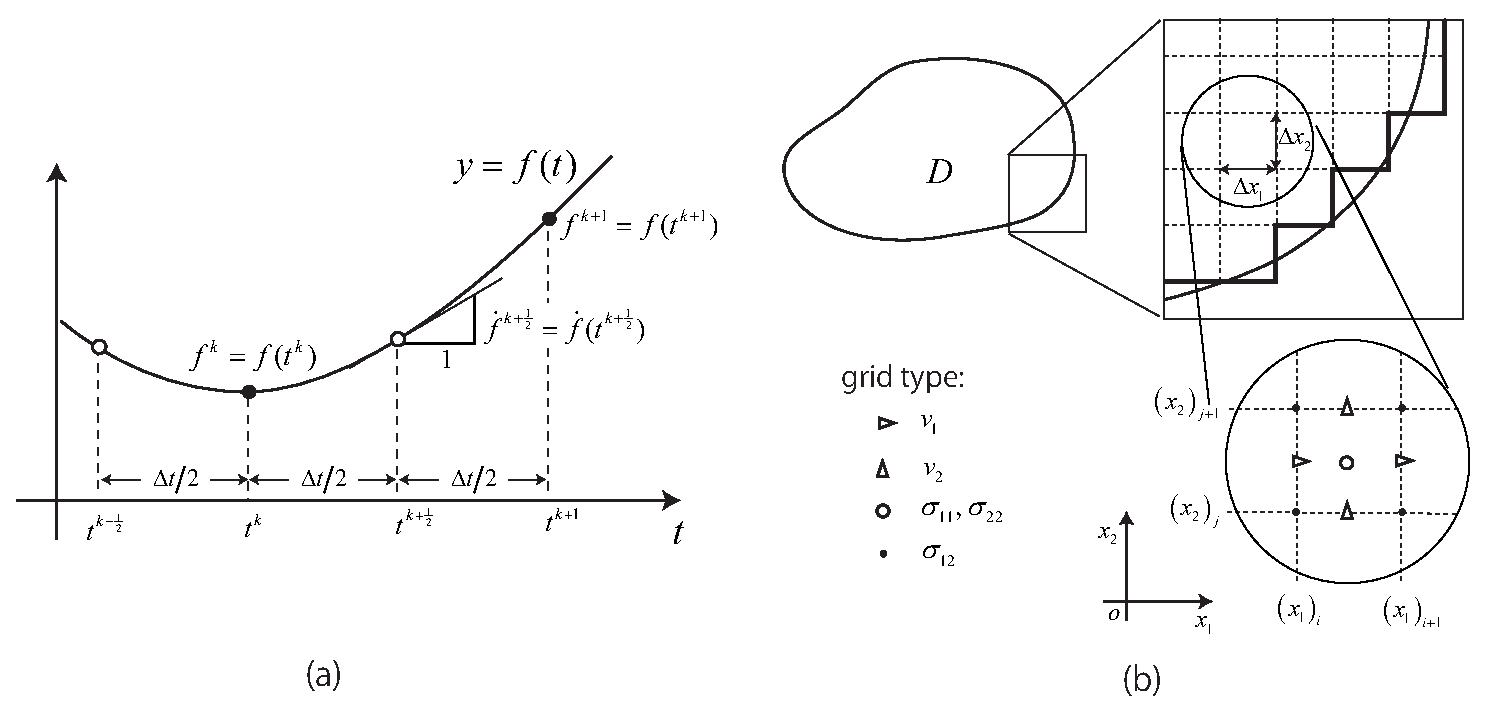
\includegraphics[width=1.0\linewidth]{Figs/FDgrid.eps}
     \end{center}
     \caption{ (a) Finite difference grid arrangement for leap-frog time stepping scheme.
	 (b) The staggered grid system for the central difference approximation 
		of spatial derivatives appearing in the governing elastoynamic 
		equations. A close-up of the unit FD-cell is also shown.
	}
     \label{fig:FDgrids}
\end{figure}
%%%%%%%%%%%%%%%%%%%%%%%%%%%
スタガード格子は図\ref{fig:FDgrids}に示したような,直応力の計算格子を中心にした
$\Delta x_1 \times \Delta x_2$の矩形領域の頂点にせん断応力の,辺上に速度の計算格子を配置したセルを基本単位とする格子配置をとる.これらの格子点における関数値を用いて, 動弾性問題の支配方程式を差分近似すれば,以下のような結果が得られる.
\begin{equation}
	\rho \frac{(v_1)_{i,j+\frac{1}{2}}^{k+1}-(v_1)^k_{i,j+\frac{1}{2}}}{\Delta t}
	=
	\frac{ 
		(\sigma_{11})^{k+\frac{1}{2}}_{i+\frac{1}{2},j+\frac{1}{2}}
		-(\sigma_{11})^{k+\frac{1}{2}}_{i-\frac{1}{2},j+\frac{1}{2}} 
	}
	{\Delta x_1}
	+
	\frac{(\sigma_{12})^{k+\frac{1}{2}}_{i,j+1}-(\sigma_{12})^{k+\frac{1}{2}}_{i,j}}{\Delta x_2}
	\label{eqn:fdtd_v1}
\end{equation}
\begin{equation}
	\rho \frac{(v_2)_{i+\frac{1}{2},j}^{k+1}-(v_2)^k_{i+\frac{1}{2},j}}{\Delta t}
	=
	\frac{(\sigma_{12})^{k+\frac{1}{2}}_{i+1,j}-(\sigma_{12})^{k+\frac{1}{2}}_{i,j}}{\Delta x_1}
	+
	\frac{ 
		(\sigma_{22})^{k+\frac{1}{2}}_{i+\frac{1}{2},j+\frac{1}{2}}
		-(\sigma_{22})^{k+\frac{1}{2}}_{i+\frac{1}{2},j-\frac{1}{2}} 
	}
	{\Delta x_2}
	\label{eqn:fdtd_v2}
\end{equation}
\begin{equation}
	\frac{
		 (\sigma_{11})^{k+\frac{1}{2}}_{i+\frac{1}{2},j+\frac{1}{2}}
		-
		 (\sigma_{11})^{k-\frac{1}{2}}_{i+\frac{1}{2},j+\frac{1}{2}}
	}
	{\Delta t}
	=
	\left( \lambda+2\mu \right)
	\frac{
		(v_1)^{k}_{i+1,j+\frac{1}{2}} - (v_1)^{k}_{i,j+\frac{1}{2}} 
	}
	{\Delta x_1}
	+
	\lambda
	\frac{
		(v_2)^{k}_{i+\frac{1}{2}, j+1} - (v_2)^{k}_{i+\frac{1}{2},j} 
	}
	{\Delta x_2}
	\label{eqn:fdtd_s11}
\end{equation}
\begin{equation}
	\frac{
		 (\sigma_{22})^{k+\frac{1}{2}}_{i+\frac{1}{2},j+\frac{1}{2}}
		-
		 (\sigma_{22})^{k-\frac{1}{2}}_{i+\frac{1}{2},j+\frac{1}{2}}
	}
	{\Delta t}
	=
	\lambda
	\frac{
		(v_1)^{k}_{i+1,j+\frac{1}{2}} - (v_1)^{k}_{i,j+\frac{1}{2}} 
	}
	{\Delta x_1}
	+
	\left( \lambda+2\mu \right)
	\frac{
		(v_2)^{k}_{i+\frac{1}{2}, j+1} - (v_2)^{k}_{i+\frac{1}{2},j} 
	}
	{\Delta x_2}
	\label{eqn:fdtd_s22}
\end{equation}
\begin{equation}
	\frac{
		 (\sigma_{12})^{k+\frac{1}{2}}_{i,j}
		-
		 (\sigma_{12})^{k-\frac{1}{2}}_{i,j}
	}
	{\Delta t}
	=
	\mu \left(
		\frac{
			(v_2)^{k}_{i+\frac{1}{2},j}
			-
			(v_2)^{k}_{i-\frac{1}{2},j}
		}
		{\Delta x_1}
		+
		\frac{
			(v_1)^{k}_{i,j+\frac{1}{2}}
			-
			(v_1)^{k}_{i,j-\frac{1}{2}}
		}
		{\Delta x_2}
	\right)	
	\label{eqn:fdtd_s12}
\end{equation}
以上の式のうち,式(\ref{eqn:fdtd_v1})から(\ref{eqn:fdtd_v2})を,$(v_1)^{k+1}_{i,j+\frac{1}{2}}$や$(v_2)^{k+1}_{i+\frac{1}{2},j}$について解けば, 速度と応力を交替に求める蛙飛び差分スキームによる差分公式が得られる.なお,以上の結果は領域内部にある計算格子において適用可能なものであるため,境界上のグリッドについては,指定された境界条件を反映した差分方程式を用いる必要がある.ここでは,トラクションが与えられた境界における境界条件の与え方について述べる.いま,計算領域を差分セルの集合で近似することを考えると,境界上に配置される可能性のある計算格子は$v_1, v_2$および$\sigma_{12}$である.このうち$\sigma_{12}$については,与えらえた境界値をそのまま代入すればよい.一方,速度$v_1, v_2$については,単位セルサイズが半分になったものと考え,運動方程式を有限体積法の考え方に従って離散化すれば,次のような差分方程式が得られる.
\begin{equation}
	\rho \frac{(v_1)_{i,j+\frac{1}{2}}^{k+1}-(v_1)^k_{i,j+\frac{1}{2}}}{\Delta t}
	=
	\alpha
	\frac{ 
		(\bar\sigma_{11})^{k+\frac{1}{2}}_{i,j+\frac{1}{2}}
		-(\sigma_{11})^{k+\frac{1}{2}}_{i-\frac{\alpha}{2},j+\frac{1}{2}} 
	}
	{\Delta x_1/2}
	+
	\frac{(\bar \sigma_{12})^{k+\frac{1}{2}}_{i,j+1}-(\bar \sigma_{12})^{k+\frac{1}{2}}_{i,j}}{\Delta x_2}
	\label{eqn:fdtd_v1_bnd}
\end{equation}
\begin{equation}
	\rho \frac{(v_2)_{i+\frac{1}{2},j}^{k+1}-(v_2)^k_{i+\frac{1}{2},j}}{\Delta t}
	=
	\frac{(\bar\sigma_{12})^{k+\frac{1}{2}}_{i+1,j}-(\bar\sigma_{12})^{k+\frac{1}{2}}_{i,j}}{\Delta x_1}
	+
	\beta
	\frac{ 
		(\bar \sigma_{22})^{k+\frac{1}{2}}_{i+\frac{1}{2},j}
		-(\sigma_{22})^{k+\frac{1}{2}}_{i+\frac{1}{2},j-\frac{\beta}{2}} 
	}
	{\Delta x_2/2}
	\label{eqn:fdtd_v2_bnd}
\end{equation}
ただし,$\bar{(\cdot)}$は既知の境界値であることを意味し,式(\ref{eqn:fdtd_v1_bnd})と(\ref{eqn:fdtd_v2_bnd})に含まれるパラメータ$\alpha$および$\beta$は,
 \begin{equation}
	\alpha=(n_1)_{i,j+\frac{1}{2}}, \ \ \beta=(n_2)_{i+\frac{1}{2},\, j},
	\label{eqn:def_ab}
\end{equation}
で,外向き法線ベクトル$\fat{n}=(n_1,\, n_2)$の方向により1または-1をとる.以上を用いて,弾性波の2次元伝播散乱解析を行った結果を次節に示す.
%%%%%%%%%%

\chapter{シミュレーション結果}
	\chapter{シミュレーション結果}
この章では、典型的な数値シミュレーション結果を示し,板や継手内部をどのように超音波が伝播するかを示す。
はじめに、もっとも基本的なケースである、板内部や表面の波動伝播挙動を示し、モード変換や散乱波の発生状況
について説明する。次に、T字継手を対象とした解析結果を、溶接ビードの形状を考慮しない場合とした場合の
二通りについて見る。これにより、溶接ビードが存在して継手部の形状が若干異なることで、波動伝播にどのような
違いが現れるかを調べる。これらの結果が超音波探傷試験の観点からどのような意味を持つかについては、
次の章で議論する。
\section{平板における波動伝播挙動}
解析モデルを図\ref{fig:}に示す.
このモデルは12mmの厚さの十分に大きな板を想定したもので、その70mmの範囲を解析対象としている。
板両端部の打ち切り位置外側にはPML(perfectly matched layer)吸収領域を設け、無反射条件を課す.
板の上下面は、送信位置以外では、トラクションゼロの境界条件を与えた.
入射波は、平板上面に鉛直力を幅1mmの範囲(4.5$\leq x \leq $5.5)mmに加えて励起した。
その際、鉛直力の時間変化はガウス分布で振幅変調した余弦波で与え、周波数は5MHzとした.
き裂は,水平方向の位置は$x=-12mm$とし,長さ4mm,角度は水平方向から15度とした.
\subsection{入射波の挙動}
図\ref{fig:fig3_1}に,き裂が存在しない場合に生じる波動場、すなわち入射場の様子を示す.
この図は、速度場$\fat{v}(\fat{x},t)$の5つの時刻におけるスナップショットを示し,横軸は
$x$、縦軸$y$とし、各点での粒子速度$\fat{v}(\fat{x},t$の絶対値をカラーマップとして表示
したものである。各々の図には、送信時からの経過時刻が示してある。また、
これらのスナップショットにあらわれている波面の内、明瞭なものについては、モードを
アルファベットで示しており、Pは縦波を、Sは横波、Hはヘッド波,Rは表面波を表している。
(a)にあるように、鉛直力を表面に加えたことで、P波が鉛直方向に強い振幅を持って励起されて
最も早く進展し、その後を、横波S波が続いている。
これらの波面形状は同心円状だが、指向性は異なり、横波はおよそ45度の方向に強く、
鉛直方向で非常に弱い。また、縦波と横波のは波面を結ぶように直線的な波面が認められ、
このような波はヘッド波といわれている。これらの波が進展すると、(b)の図にあるように
板表面近傍に強い表面波(レイリー波)が発生し、横波と分離して現れるようになる。
これら4種類の波は、半無限領域表面に鉛直力を加えたときに発生する波と同じもので、
Lambの解によって理論的に存在と挙動が説明されている。
P波は、(b)に示した時刻では板の下面に達して反射している。
反射の際、P波はP波とS波の両方を発生させる。
この図ではP波の反射によって発生したP波をP-P, P波の反射じにモード変換してS波に転じたものをP-S
として示している。P波は鉛直入射したもの以外は、P、S両方のモードの波を発生させ、
P-Pの後を、伝播速度の遅いP-S波が追いかける形になっている。
(c)では、S波が下面に達した直後の状況を示している。S波についても、P、S両方の反射波
が発生している。この様子は更に時間が経過した(d)の図でより明確であるため、(d)には
S-PとS-Sの波面の所在を示している。なお、(c)ではP波、はやくも2回目の反射を板上面で
起こしており、あまり振幅を低下させることなく伝播していることが分かる。
このように、P波はおよそS波の2倍程度の位相速度で進行するため、S波を追い越しながら
伝播する.(e)にもあるように、板内部では、P波、S波とも、モード変換を伴いつつ、
多重反射を起こすため、板のように単純な形をした部材内部でも、かなり複雑な波動場を
形成する。なお、このような多順反射波が十分な回数繰り返されて干渉を起こす結果が
ガイド波である。ここでの計算条件では、P波の波長が約1.2mm、横波波長が約0.6mm
で、板厚に比べて小さいため、ガイド波が形成されるまでには非常に長い時間が必要とされる
ために、超音波探傷で問題となる観測時間の範囲においては、ガイド波としての解析や解釈
はほとんど意味をなさない。
%--------------------
\begin{figure}[h]
	\begin{center}
	\includegraphics[width=0.8\linewidth]{Figs/plate_inc.eps} 
	\end{center}
	\caption{
		速度場$|\fat{v}(\fat{x},t)|$のスナップショット.
		P,Sは縦波,横波を,Rは表面波,Hはヘッド波を表す.
		ハイフンで繋がれた文字は反射前後でのモードを表す. き裂が存在しない場合.
	} 
	\label{fig:fig3_1}
\end{figure}
\begin{figure}[h]
	\begin{center}
	\includegraphics[width=0.8\linewidth]{Figs/plate_tot.eps} 
	\end{center}
	\caption{
		速度場$|\fat{v}(\fat{x},t)|$のスナップショット.
		P,Sは縦波,横波を,Rは表面波,Hはヘッド波を表す.
		き裂がある場合.
	} 
	\label{fig:fig3_2}
\end{figure}
\begin{figure}[h]
	\begin{center}
	\includegraphics[width=0.8\linewidth]{Figs/plate_sct.eps} 
	\end{center}
	\caption{
		速度場$|\fat{v}(\fat{x},t)|$のスナップショット.
		P,Sは縦波,横波を,Rは表面波,Hはヘッド波を表す.
		き裂がある場合の散乱波成分のみを表示.
	} 
	\label{fig:fig3_3}
\end{figure}
\begin{figure}[h]
	\begin{center}
	\includegraphics[width=0.8\linewidth]{Figs/plate_bwvs.eps} 
	\end{center}
	\caption{
		$x=0\sim35, y=12$mmの位置で得られた波形の走時プロット.
		(a)き裂なし,(b)き裂ありの場合.
		(c)はき裂ありと無しの場合の差分をとって計算した散乱波成分.
	} 
	\label{fig:fig3_4}
\end{figure}
%--------------------
\section{T字継手における波動伝播挙動(余盛り形状を考慮しない場合)}
%--------------------
\begin{figure}[h]
	\begin{center}
	\includegraphics[width=1.0\linewidth]{Figs/T_inc.eps} 
	\end{center}
	\caption{
		速度場$|\fat{v}(\fat{x},t)|$のスナップショット.
		P,Sは縦波,横波を,Rは表面波,Hはヘッド波を表す.
		ハイフンで繋がれた文字は反射前後でのモードを表す. き裂が存在しない場合.
	} 
	\label{fig:fig3_5}
\end{figure}
\begin{figure}[h]
	\begin{center}
	\includegraphics[width=1.0\linewidth]{Figs/T_tot.eps} 
	\end{center}
	\caption{
		速度場$|\fat{v}(\fat{x},t)|$のスナップショット.
		P,Sは縦波,横波を,Rは表面波,Hはヘッド波を表す.
		き裂がある場合.
	} 
	\label{fig:fig3_6}
\end{figure}
\begin{figure}[h]
	\begin{center}
	\includegraphics[width=1.0\linewidth]{Figs/T_sct.eps} 
	\end{center}
	\caption{
		速度場$|\fat{v}(\fat{x},t)|$のスナップショット.
		P,Sは縦波,横波を,Rは表面波,Hはヘッド波を表す.
		き裂がある場合の散乱波成分のみを表示.
	} 
	\label{fig:fig3_7}
\end{figure}
\begin{figure}[h]
	\begin{center}
	\includegraphics[width=1.0\linewidth]{Figs/T_bwvs.eps} 
	\end{center}
	\caption{
		$x=0\sim35, y=12$mmの位置で得られた波形の走時プロット.
		(a)き裂なし,(b)き裂ありの場合.
		(c)はき裂ありと無しの場合の差分をとって計算した散乱波成分.
	} 
	\label{fig:fig3_8}
\end{figure}
%--------------------



\chapter{継手ディテールを考慮した超音波伝播シミュレーション}
	\chapter{超音波探傷の観点からの考察}
\begin{figure}[h]
	\begin{center}
	\includegraphics[width=1.0\linewidth]{Figs/bead_inc.eps} 
	\end{center}
	\caption{
		速度場$|\fat{v}(\fat{x},t)|$のスナップショット.
		P,Sは縦波,横波を,Rは表面波,Hはヘッド波を表す.
		ハイフンで繋がれた文字は反射前後でのモードを表す. き裂が存在しない場合.
	} 
	\label{fig:fig4_1}
\end{figure}
\begin{figure}[h]
	\begin{center}
	\includegraphics[width=1.0\linewidth]{Figs/bead_tot.eps} 
	\end{center}
	\caption{
		速度場$|\fat{v}(\fat{x},t)|$のスナップショット.
		P,Sは縦波,横波を,Rは表面波,Hはヘッド波を表す.
		き裂がある場合.
	} 
	\label{fig:fig4_2}
\end{figure}
\begin{figure}[h]
	\begin{center}
	\includegraphics[width=1.0\linewidth]{Figs/bead_sct.eps} 
	\end{center}
	\caption{
		速度場$|\fat{v}(\fat{x},t)|$のスナップショット.
		P,Sは縦波,横波を,Rは表面波,Hはヘッド波を表す.
		き裂がある場合の散乱波成分のみを表示.
	} 
	\label{fig:fig4_3}
\end{figure}
\begin{figure}[h]
	\begin{center}
	\includegraphics[width=1.0\linewidth]{Figs/bead_bwvs.eps} 
	\end{center}
	\caption{
		$x=0\sim35, y=12$mmの位置で得られた波形の走時プロット.
		(a)き裂なし,(b)き裂ありの場合.
		(c)はき裂ありと無しの場合の差分をとって計算した散乱波成分.
	} 
	\label{fig:fig4_4}
\end{figure}
%--------------------



%--------------------
\chapter{結論と今後の課題}
本研究では,不飽和粘土の電気化学インピーダンス特性を把握することを目的として,
モンモリロナイトを圧縮成形して作成した供試体を用いてインピーダンススペクトル
の計測を行った. インピーダンス計測は,粘土供試体の含水比と乾燥密度が異なる場合
について行い,水分量とかさ密度の影響を調べた,また,計測結果を再現する
ための等価回路を設定して回路定数の推定を行い,回路定数と水分,密度の関係について
検討を行った.その結果として得られた知見は以下のようである.
\begin{enumerate}
\item
        圧縮成形された粘土供試体のインピーダンススペクトルは低周波側で容量性の半円を示す.
        ただし,その半円は実数軸方向に扁平な形状とり,高周波側では45度よりも大きな
	傾きの直線的変化を示す.
\item
	上記の特徴を捉えたインピーダンススペクトルは,Cole-Coleプロットで与えることができる.
	Cole-Coleプロットの等価回路は,CPEと抵抗の並列回路に別の抵抗を直列接続した直−並列回路
	で与えられる.
\item
	直列接続された抵抗$R_{0}$は供試体内の直流成分に関する電荷移動抵抗を,
	並列接続された抵抗$R_{ct}$は物質界面での電荷移動抵抗を表し,
	CPEは局所的な分極(電気二重層)の発生による蓄電効果を表現する.
\item
	実験結果から推定した等価回路の回路定数のうち,直列抵抗成分$R_{ct}$とCPEの時定数
	$T_{CPE}$およと指数$p$は,含水比と乾燥密度との間に相関を示す.
\item
        直列抵抗成分$R_{ct}$は含水比,乾燥密度の増加にいずれに対しても減少する.
\item
        $T_{CPE}$は含水比の増加につれて大きくなる.このことは局所的な分極は間隙水中で
	生じていることを意味する.
\item
        $T_{CPE}$は乾燥密度の増加に対しても増加し,これは局所的な分極が密度が
	高いほど,より狭い範囲に集中することに起因する.
\item
        CPEの指数$p$は含水比$20\%$程度で最大となり,もっともコンデンサーに近い応答を示す.
        乾燥密度との関係では,水分量が少ないときには密度の増加に対して$p$が増加するが,
        水分量が多いときには密度の増加にたいして指数$p$は減少する.
\item
        指数$p$のこのような振る舞いには,水分や空隙の量だけでなくその構造
	(連結性や屈曲率)が影響している.
\item
        $T_{CPE}$は局所的な分極による蓄電容量を,指数$p$は印加電圧に対する
	帯電量変化の位相遅れを表す.
\end{enumerate}
今後はより正確なフィッティングが可能な等価回路の推定や,回路素子定数を同定
するための効率的な非線形最小二乗法の開発が課題となる.
また,等価回路の回路素子に対応する電気化学プロセスを正確に特定し,微視構造モデルと
回路定数の定量的な関係をつけることが重要な課題となる.この点が解決されれば,
粘土鉱物スケールでの微視的な電荷移動や間隙と間隙水構造
に関する情報をインピーダンス計測結果から逆推定する道が拓ける.
\renewcommand{\bibname}{参考文献}
\begin{thebibliography}{99}
%\begin{spacing}{1.175}
\bibitem{Fujiie}
	藤家洋一: 原子力-自然に学び,自然を真似る-, ERC出版,2005.
\bibitem{NUMO_URL}
	原子力発電環境整備機構: https://www.numo.or.jp/chisoushobun/.
\bibitem{NUMO}
	原子力発電環境整備機構:地層処分事業の安全確保(2010年度版)-確かな技術による安全な地層処分の実現のために-, NUMO-TR-11-01, 2011.
\bibitem{Sudo}
	須藤談話会編, 粘土科学への招待 粘土の素顔と魅力, 三共出版, 2000.
\bibitem{Watanabe}
	T.Watanabe and T.Satou: Expansion characteristics of montmorillonite and saponite under various 
	relative humiditiy conditions, Clay Science, 7, pp.129-138, 1988.
\bibitem{Morodome}
	S.Morodome and K.Kawamura: Swelling behavior of Na- and Ca- montmorillonite up to 150$^\circ$ by in-situ 
	X-ray diffraction experiments, Clay and Clay Minerals, vol.57, No.2, pp.150-160, 2009.
\bibitem{Sato}
	佐藤努: 粘土鉱物の水和と吸着水の構造, 鉱物学雑誌, 第25巻, 第3号 , pp.99-110, 1996.
\bibitem{ieItagaki}
	板垣 昌幸:電気化学インピーダンス法 第二版 原理・測定・解析,丸善出版, 2011. 
%\end{spacing}
\end{thebibliography}
\end{document}
%%%%%%%%%%%%%%%%%%%%%%%%%%%%%%%%%%%%%%%%%%%%

